\documentclass[10pt,journal,final,finalsubmission,twocolumn]{IEEEtran}
%\pagestyle{empty}
%\documentclass[9.5pt,journal,final,finalsubmission,twocolumn]{IEEEtran}
%%%%%%%%\renewcommand{\baselinestretch}{2}
\usepackage{stmaryrd}
\usepackage{amsfonts}
\usepackage{url}
\usepackage{mathrsfs,amsmath}
%\usepackage{caption2} 
\usepackage{graphicx,times}
\usepackage{cleveref}
\usepackage{cite}
\usepackage{amssymb}
\usepackage{makeidx}
\usepackage{multirow}
\usepackage{subfigure}
\usepackage{algorithmic} 
%\usepackage{ntheorem}
%\usepackage[justification=centering]{caption}
\usepackage{bm}
\usepackage[ruled,linesnumbered,vlined]{algorithm2e}  
%\usepackage{caption}
%\usepackage[top=2cm, bottom=2cm, left=2cm, right=2cm]{geometry}    
\usepackage{setspace}
\usepackage{amsthm}
\usepackage{booktabs}
\usepackage{authblk}



\newtheorem{theorem}{Theorem}
\newtheorem{lemma}[theorem]{Lemma}
\newtheorem{proposition}{Proposition}
\newtheorem{definition}{Definition}
\newtheorem{corollary}[theorem]{Corollary}
\newtheorem*{pf}{Proof}


%\newenvironment{proof}{{\noindent\it Proof}\quad}{\hfill $\square$\par}



\newcommand{\tabincell}[2]{\begin{tabular}{@{}#1@{}}#2\end{tabular}}
% correct bad hyphenation here
\hyphenation{}
\IEEEoverridecommandlockouts    % to create the author's affliation portion
                % using \thanks

%\textwidth 178mm    % <------ These are the adjustments we made 10/18/2005
%\textheight 239mm   % You may or may not need to adjust these numbes again
%\oddsidemargin -7mm
%\evensidemargin -7mm
%\topmargin -6mm
%\columnsep 5mm
\renewcommand\thepage{}
%\renewcommand{\baselinestretch}{1.57}
\allowdisplaybreaks

\begin{document}

\title{Leveraging Muiti-cell NOMA for Cell Edge}

\author{Zhanwei Yu\textsuperscript{1}, Lei You\textsuperscript{2} and Di Yuan\textsuperscript{1}}
\affil{\textsuperscript{1}Department of Information Technology, Uppsala University, Sweden
\authorcr \textsuperscript{2}Independent Researcher, Sweden
\authorcr {\em Emails: zwyuapr1@gmail.com;lei.you@pm.me;di.yuan@it.uu.se}}
\renewcommand*{\Affilfont}{\small}

\maketitle
\begin{abstract}
Non-orthogonal multiple access (NOMA) is a promising technique for performance enhancement in cellular networks. This paper investigates how much NOMA can offer for cell edge in multi-cell scenarios. We consider the joint optimization problem of time-frequency resource allocation, user pairing, and power split, for scaling up the demand delivered for edge users. Our approach for problem solving consists in iteratively applying a fixed-point method to the cells, and, for each cell, deriving an algorithm guaranteeing optimum for single-cell optimization. By embedding the fixed-point method into bi-section search, we are able to show the overall approach guarantees global optimality. Numerical results demonstrate that multi-cell NOMA optimization has much more to offer over orthogonal multiple access for the experience of edge users, in particular for high-demand and resource-limited scenarios. 
\end{abstract}


\begin{keywords}
NOMA, multi-cell, cell edge, resource allocation
\end{keywords}

%-----------------------------------------------------------------------------------------------------------------------------------------------
\section{Introduction}  \label{Sec:Intro}

Designing beyond-5G systems targets squeezing more bits out of the spectrum. Non-orthogonal multiple access (NOMA) is considered a promising radio access technique for performance enhancement. The basic idea of NOMA is using the same transmission channel to simultaneously serve multiple user equipments (UEs) at the cost of inter-user interference. By utilizing successive interference cancellation (SIC), NOMA can achieve better performance than orthogonal multiple access (OMA).

The experience of edge UEs is an important performance metric. There are a number of works studying improving this metric with NOMA. In \cite{Do1}, the performance of a single edge UE in a two-user multiple-input single-output (MISO) NOMA system is studied and three cooperative downlink transmission schemes with simultaneous wireless information and power transfer (SWIPT) are proposed. To improve the experience of the edge UEs in a two-user NOMA system, the authors of \cite{Do2} propose two cooperative relaying schemes, called on/off full-duplex relaying and on/off half-duplex relaying. In \cite{Guo}, a two-cell NOMA system is considered, where two center UEs are served by their respective cells and one edge UE is served by both cells, the authors propose both centralized and distributed algorithms to minimize the total transmit power. In \cite{Pei}, the authors propose a downlink NOMA based coordinated direct and relay system with one center UE and multiple edge UEs, where a decode-and-forward and full-duplex relay is used to help the latter.

The works in \cite{Do1, Do2, Guo, Pei} all focus on single-cell or two-cell scenarios. For more general multi-cell NOMA, resource optimization is more challenging, due to the interplay between SIC and inter-cell interference.

Recently, some studies have addressed general-scenario multi-cell NOMA. The authors of \cite{Ali} consider the problem of dynamic power allocation with coordinated multi-point (CoMP) transmission in the downlink and propose a distributed power optimization approach. The authors of \cite{You1} study the cell load coupling system for multi-cell NOMA, and propose an algorithm for power allocation and UE pairing for optimal resource management. A complementary note to \cite{You1} is provided in \cite{You2}. The authors of \cite{Ni} study the total transmit power minimization problem for multi-cell and multi-carrier NOMA (MCMC-NOMA) networks, and propose a resource allocation algorithm that can dramatically reduce the power consumption. The authors of \cite{Lei} investigate energy optimization in MCMC-NOMA networks, and propose tailored algorithms to provide energy-efficient solutions for three NOMA grouping schemes.

Different from \cite{Do1, Do2, Guo, Pei}, which focus on single-cell or two-cell NOMA systems, we consider more general multi-cell scenarios. In addition, we focus on the experience of edge UEs. Indeed, the achievable rate of the edge UEs is generally much lower than that of the cell-center UEs \cite{Dai}. We aim at investigating how much NOMA can offer to edge UEs. To this end, we study the joint optimization problem of time-frequency resource allocation, UE pairing, and power split, with the objective of maximizing the amount of data delivered to cell-edge UEs. We formulate this problem and derive its fundamental properties. We first propose a single-cell algorithm, aiming to minimize time-frequency resource consumption for any given amount of data to be delivered to the edge UEs within one cell, while the resource allocation of other cells is tentatively fixed. Next, we iteratively apply a fixed-point method with the single-cell algorithm to minimize multi-cell resource consumption. Then, we approach the global optimum of the overall problem by embedding the fixed-point method into bi-section search. Finally we evaluate the performance of the algorithm in multi-cell NOMA compared to OMA.

%-----------------------------------------------------------------------------------------------------------------------------------------------
\section{System Model and Problem Formulation} \label{Sec:SystemModel}

\subsection{System Model}\label{Preliminaries}

Denote by $\mathcal{I} = \{1,2,...,I \}$ and $\mathcal{J} = \{1,2,...,J\}$ the sets of cells and UEs, respectively. 
We consider downlink and denote by $g_{ij}$ the channel power gain from cell $i$ to UE $j$ $(i \in \mathcal{I}, j \in \mathcal{J})$. Denote by $\mathcal{J}_i$ the set of UEs served by cell $i$.

The time-frequency resource is divided into resource units (RUs). In NOMA, multiple UEs can access the same RU by SIC. However, the complexity of decoding grows rapidly with the number of UEs involved in SIC. It has been demonstrated that two UEs in SIC can offer a good trade-off between complexity and performance \cite{Islam}. In view of this, we consider two UEs in one cell sharing one RU as a {\em pair} (denoted by $u=\{j,h\}$), and call the process of selecting UEs to form pairs as {\em UE pairing} or simply {\em pairing}. To keep the generality, a pair may consist of a single UE $j$, i.e., UE uses the OMA mode, and we denote this special pair by $u=\{0,j\}$. For cell $i$, denote by $\mathcal{U}_i$ the set of all candidate pairs of UEs in $\mathcal{J}_i$. Similarly, use $\mathcal{U}_j$ to refer to the set of all pairs containing UE $j$. Furthermore, we use ${\mathcal{U}}$ to refer to the set of all candidate pairs, i.e., $\mathcal{U} = \bigcup _{i \in \mathcal{I}}  \mathcal{U}_i$, and use $N$ to denote the cardinality of U, i.e., $N=|\mathcal{U}|$. Also, we put indices on $u$ to differentiate between the pairs, i.e., $\mathcal{U} = \{u_1,u_2,...,u_N\}$. We use a binary $y_{u}$ to indicate whether or not the pair $u$ is selected. We optimize pairing by optimizing $\boldsymbol{y}$, where $\boldsymbol{y} = [y_{u_1},y_{u_2},...,y_{u_N}]$.

We use $p_i$ to denote the transmission power of cell $i$ on an RU. For each pair $u$ in cell $i$, {\em power splitting} is done on $p_i$, with $q_{ju}$ and $q_{hu}$ allocated to UE $j$ and $h$, respectively. Namely,
\begin{equation}
p_i = q_{ju} + q_{hu}.
\end{equation}
Besides, denote by $x_u$ the proportion of RUs allocated to pair $u$. We have
 \begin{equation}
 \rho_i = \sum \nolimits_{u \in {\mathcal{U}}_i} x_u \leq \bar{\rho},  i\in \mathcal{I},
 \end{equation}
where $\bar{\rho}$ is how many RUs at most can be allocated in one cell. 

%We remark that we obtain optimal pairs by optimizing $\boldsymbol{x} = [x_{u_1},x_{u_2},...,x_{u_N}]$ and the optimal $\boldsymbol{x}^*$ also represents the result of pairing optimization. If any $x_u^* > 0$, UEs $j$ and $h$ form a pair $u$ to share RU in NOMA mode, and if $x_u^* = 0$, then UEs $j$ and $h$ ($j,h \in u$) do not share RU.

For any UE $j$ $\left(j \in u\right)$, the signal-to-interference and noise ratio (SINR) is computed by
\begin{equation}
\gamma _{ju} \!=\!\frac{q_{ju}g_{ij}}{{B_{ju}q_{hu}g_{ij}}\!+\!{\sum_{k\in \mathcal{I}\setminus \left \{ i \right \}}p_kg_{kj}\rho_k}\!+\!\sigma ^2}, j\!\in\! u, u \!\in\!{\mathcal{U}}.\label{1111}
\end{equation}
We set $\gamma_{0u} = 0$ to for with the special case $u=\{0,j\}$.

In (\ref{1111}), $B_{ju}q_{hu}g_{ij}$ is the inter-user interference within a cell due to SIC, where $B_{ju}$ is a binary indicator depending on $j$'s decoding order. If UE $j$ decodes $h$'s signal first and hence $h$'s signal does not affect $j$, $B_{ju} = 0$, otherwise, $B_{ju} = 1$. Besides, ${\sum_{k\in \mathcal{I}\setminus \left \{ i \right \}}p_kg_{kj}\rho_k}$ is the inter-cell interference, where $\rho_k$ is the amount of time-frequency resource consumption of cell $k$ and reflects the likelihood that a UE outside cell $k$ receives interference from $k$. The symbol $\sigma^2$ is the noise power.

In addition, in any pair $u$, the optimal decoding order (i.e., $B_{ju}$ and $B_{hu}$) is determined by the channel condition, inter-cell interference, and noise \cite{41}. We define $w_j$ for the purpose of modeling the decoding order for any UE $j$ as follows. 
\begin{equation}
w_j=  \left(\sum \limits_{k \in \mathcal{I}\setminus \left \{ i \right \} }p_k g_{kj}\rho_k+\sigma ^2   \right) / g_{ij} .
\end{equation}
In NOMA, the UE, which has better received signal in relation to inter-cell interference and noise, decodes the other UE in a pair first and there is no inter-user interference in its denominator of SINR. Thus, in any pair $u$, we have the following rule. 
\begin{equation}\label{rule}
\left\{\begin{array}{l}
B_{ju} = 0,B_{hu} =1, \text{if } w_j < w_h,\\
B_{ju} = 1,B_{hu} =0, \text{otherwise}.
\end{array}\right.
\end{equation}
For the special case of $u = \{0, j\}$, the value of $w_0$ is set to be a large value such that in effect UE $j$ is in the OMA mode.

According to (\ref{1111}), we can obtain the achievable capacity for UE $j$ in pair $u$ on any RU as follows, where $\boldsymbol{q}=[q_{ju_1},q_{hu_1},q_{ju_2},q_{hu_2},...,q_{ju_N},q_{hu_N},]$, $\boldsymbol{\rho}=[\rho_1,\rho_2,..., \rho_I]$, and $\boldsymbol{B}=[B_{ju_1},B_{hu_1},B_{ju_2},B_{hu_2},...,B_{ju_N},B_{hu_N},]$.
\begin{align}\label{cju0}
c_{ju}\left (\boldsymbol{q},\boldsymbol{ \rho}, \boldsymbol{B}\right )\!=\!\log \left ( 1\!+\!\gamma_{ju} \right )\!=\!\log \Big ( 1\!+\!\frac{q_{ju}}{B_{ju}q_{hu}\!+\!w_j} \Big )\notag\\
=\!\log \bigg ( 1+\frac{q_{ju}g_{ij}}{{B_{ju}q_{hu}g_{ij}}\!+\!{\sum_{k\in \mathcal{I}\setminus \left \{ i \right \}}p_kg_{kj}\rho_k}\!+\!\sigma ^2} \bigg ).
\end{align}
We use $d_j$ to denote the base demand of UE $j$ ($j \in \mathcal{J}$) and denote by $M$ and $B$ the total number of RUs in one cell and the bandwidth of each RU, respectively. We have
\begin{equation}
\sum\nolimits_{u\in {\mathcal{U}}_j} M B c_{ju}\left (\boldsymbol{q},\boldsymbol{ \rho}, \boldsymbol{B}\right )x_u\geq d_j, j \in \mathcal{J}.
\end{equation}
In addition, we use $\mathcal{S}$ to denote the set of edge UEs. We would like to scale up the demand that can be delivered to the edge UEs by a {\em scaling factor} $\alpha$ $\left (\alpha \geq 1\right)$ because considering the maximization of $\alpha$ can tell us how much NOMA can offer to edge UEs. Thus, we have
\begin{equation}
\sum\nolimits_{u\in {\mathcal{U}}_j} M B c_{ju}\left (\boldsymbol{q},\boldsymbol{ \rho}, \boldsymbol{B}\right )x_u\geq \alpha d_j,j\in \mathcal{S}.
\end{equation}

For convenience, in the following discussion, we use normalized $d_j$ such that two notations $M$ and $B$ are not necessary.

\subsection{Problem Formulation}\label{MathematicalFormulation}

Consider optimizing resource allocation in NOMA networks for demand scaling maximization of edge UEs. We optimize power split $\boldsymbol{q}$, pair-level resource allocation $\boldsymbol{x}$, pair selection $\boldsymbol{y}$, decoding order indicator $\boldsymbol{B}$, and cell-level resource allocation $\boldsymbol{\rho}$. The objective function $\alpha$ is the scaling factor for the given set of edge UEs $\mathcal{S}$ ($\mathcal{S}\subseteq \mathcal{J}$), with respect to the base UE demand $\boldsymbol{d}=[d_1,d_2,...,d_m]$. The formulation is in (\ref {formulation}).
\begin{subequations}\label{formulation}
\begin{align}
\textup{[{\em MaxD}]}&\ \ \ \ \ \ \ \ \ \ \ \ \ \ \ \ \ \ \underset{\alpha \geq 1,\boldsymbol{q},\boldsymbol{x},\boldsymbol{\rho}\geq \boldsymbol{0} }{\max} \alpha  \\
\textup{ s.t.}& \sum\limits_{u\in {\mathcal{U}}_j} c_{ju}\left (\boldsymbol{q},\boldsymbol{ \rho}, \boldsymbol{B}\right )x_u\geq \alpha d_j, j\in \mathcal{S}\label{demand1}\\ 
& \sum\limits_{u\in {\mathcal{U}}_j} c_{ju}\left (\boldsymbol{q},\boldsymbol{ \rho}, \boldsymbol{B}\right )x_u\geq  d_j, j\in \mathcal{J} \setminus  \mathcal{S}\label{demand2}\\ 
&\sum \limits_{j \in u} q_{ju}\leq p_i,u\in {\mathcal{U}}_i, i\in \mathcal{I}  \label{limit1}\\
&\rho _i =\sum \limits_{u\in {\mathcal{U}}_i}x_u\leq \bar{\rho}, i\in \mathcal{I} \label{limit2}\\
&x_u\leq y_u \bar{\rho}, u\in \mathcal{U}\label{y1}\\
&\sum\limits_{u\in \mathcal{U}_j}y_u\leq1,j\in\mathcal{J}\label{y2}\\
&y_u\in\{0,1\}, u\in \mathcal{U}\label{y3}\\
&w_j\!=\!  \frac{\left(\sum \nolimits_{k \in \mathcal{I}\setminus \left \{ i \right \} }p_k g_{kj}\rho_k+\sigma ^2   \right)}{ g_{ij}},j \in \mathcal{J}_i ,i\in \mathcal{I}\label{order0}\\
&w_j>w_h\vee(w_j=w_h\wedge h < j)\Rightarrow B_{ju}=1,\notag\\
&\ \ \ \ \ \ \ \ \ \ \ \ \ \ \ \ \ \ \ \ \ \ j\neq h,j,h\in u, u\in \mathcal{U}_i, i\in \mathcal{I}\label{order1}\\
&B_{ju}+B_{hu}=1, j\neq h, j,h\in u, u\in \mathcal{U}_i, i\in \mathcal{I}\label{order2}\\
&B_{ju},B_{hu}\in\{0,1\}, j,h \in u, u\in \mathcal{U}\label{order3}
\end{align}
\end{subequations}



The UEs in $\mathcal{S}$ can be regarded as being throughput-oriented such that delivering more bits leads to higher satisfaction, as imposed by constraints (\ref{demand1}). Constraints (\ref{demand2}) guarantee other UEs $j$ $(j \!\in \!\mathcal{J} \!\setminus\mathcal{S})$ meet their demand $d_j$. Constraints (\ref{limit1}) and (\ref{limit2}) impose the cell power limit and RU limit of any cell, respectively. Constraints (\ref{y1}) guarantee that RU allocation occurs only for selected pairs. By constraints (\ref{y2}) and (\ref{y3}), each UE belongs up to one pair such that the selected pairs are not overlapping. Constraints (\ref{order0}) - (\ref{order3}) are for the decoding order in a pair, and they make decoding orders follow the rule (\ref{rule}) in Section II-A. 



%----------------------------------------------------------------------------------------------------------------------------
\section{Fundamental Properties of MaxD} \label{Sec:properties}

Before presenting the solution method for {\em MaxD}, we outline two lemmas for optimality characterization. The lemmas provide some fundamental properties for solving {\em MaxD}. 


We denote by $\mathcal{H}$ a function that gives the normalized maximum time-frequency resource consumption of one cell, i.e.,
\begin{equation}
\mathcal{H}(\boldsymbol{\rho}) = \frac{1}{\bar{\rho}}\underset{i\in \mathcal{I}}{\max} \ \rho_i.
\end{equation}


\begin{lemma}\label{property 1}
$[\alpha ^*, \boldsymbol{q}^*,\boldsymbol{x}^*,\boldsymbol{\rho}^*, \boldsymbol{y}^*, \boldsymbol{B}^*]$ is optimal to MaxD, only if $\mathcal{H}(\boldsymbol{\rho^*}) = 1$.
\end{lemma}
\begin{proof} 
Obviously any solution with $\mathcal{H}(\boldsymbol{\rho}) > 1$ is infeasible because at least one of (\ref{limit2}) is violated. Now consider an optimal solution and suppose $\mathcal{H^*}(\boldsymbol{\rho}) < 1$. We increase $\boldsymbol{x}^*$ to $\boldsymbol{x}' =\beta\boldsymbol{x}^*$ $(\beta >1)$ such that $\boldsymbol{\rho}' =\beta\boldsymbol{\rho}^*$ satisfies $\mathcal{H}(\boldsymbol{\rho}') =1$. To show doing so is feasible, we first define an auxiliary function $g(z) = (1+\frac{z}{\beta})^\beta$. According to Taylor's formula, the auxiliary function can be written as
\begin{equation}\label{goto}
g(z) =(1+\frac{z}{\beta})^\beta=1+z+R_1(z)>1+z,
\end{equation}
where $R_1(z)=\frac {(\beta-1)(1+\frac{\theta z}{\beta})^{\beta-2}(\theta z)^2}{2\beta}>0$ $(\theta \in (0,1))$, which is the Lagrange remainder. For each UE $j$ $(j\in \mathcal{S})$, with (\ref{goto}) we thus have
\begin{align}
&\sum\limits_{u\in \mathcal{U}_j} c_{ju}\left (\boldsymbol{q}^*,\boldsymbol{ \rho}', \boldsymbol{B}^*\right ) x_u'=\sum\limits_{u\in \mathcal{U}_j} c_{ju}\left (\boldsymbol{q}^*,\beta\boldsymbol{ \rho}^*, \boldsymbol{B}^*\right ) \beta x_u^*\notag\\
=&\sum\limits_{u\in \mathcal{U}_j}\!\beta\log \bigg ( 1\!+\!\frac{q_{ju}^*g_{ij}}{{B_{ju}^*q_{hu}^*g_{ij}}\!+\!\beta{\sum\nolimits_{ k\in \mathcal{I}\setminus \left \{ i \right \}}p_kg_{kj}\rho_k^*}\!+\!\sigma ^2} \bigg ) x_u^*\notag\\
>& \sum\limits_{u\in \mathcal{U}_j}\!\log \Bigg [ 1\!+\!\frac{q_{ju}^*g_{ij}}{\beta\big({B_{ju}^*q_{hu}^*g_{ij}}\!+\!{\sum\nolimits_{k\in \mathcal{I}\setminus \left \{ i \right \}}p_kg_{kj}\rho_k^*}\!+\!\sigma ^2\big)} \Bigg ]^\beta \!x_u^*\label{lemma1-1}\notag\\
>&\sum\limits_{u\in \mathcal{U}_j}\!\log \bigg ( 1\!+\!\frac{q_{ju}^*g_{ij}}{\!\!{B_{ju}^*q_{hu}^*g_{ij}}\!+\!{\sum\nolimits_{k\in \mathcal{I}\setminus \left \{ i \right \}}p_kg_{kj}\rho_k^*}\!+\!\sigma ^2} \bigg ) x_u^*\notag\\
=&\!\sum\limits_{u\in \mathcal{U}_j} c_{ju}\left (\boldsymbol{q}^*,\boldsymbol{ \rho}^*, \boldsymbol{B}^*\right )  x_u^*\geq\alpha d_j\notag\\
\ &\ \ \ \ \ \ \ \ \ \ \ \Rightarrow \sum\limits_{u\in \mathcal{U}_j} c_{ju}\left (\boldsymbol{q}^*,\boldsymbol{ \rho}', \boldsymbol{B}^*\right ) x_u'>\alpha d_j
\end{align}

The same process applies for UE $j$ $(j\in \mathcal{J}\setminus\mathcal{S})$. Therefore, $\boldsymbol{\rho}'$ is a feasible solution to {\em MaxD} such that all inequalities in (\ref{demand1}) and (\ref{demand2}) strictly hold. Under $\boldsymbol{\rho}'$, one can increase $\alpha^*$ to $\alpha '$ such that at least one of (\ref{demand1}) holds as equality, to obtain a better objective value, which contradicts the assumption that $[\alpha^*, \boldsymbol{q}^*,\boldsymbol{x}^*,\boldsymbol{\rho}^*, \boldsymbol{y}^*,\boldsymbol{B}^*]$ is optimal. Hence the conclusion.
\end{proof}

By Lemma \ref{property 1} we know that a solution is optimal to (\ref{formulation}) only if there exists at least one cell that uses all the time-frequency resource. Intuitively, if all cells have unused time-frequency resource, then one can improve the objective function such that more data would be delivered to UEs. 

\begin{lemma}\label{property 2}
$[\alpha ^*, \boldsymbol{q}^*,\boldsymbol{x}^*,\boldsymbol{\rho}^*, \boldsymbol{y}^*,\boldsymbol{B}^*]$ is optimal to MaxD, only if (\ref{demand1}) and (\ref{demand2}) all hold as equality.
\end{lemma}
\begin{proof}
Consider an optimal solution to {\em MaxD}, denoted by $[\alpha ^*, \boldsymbol{q}^*,\boldsymbol{x}^*,\boldsymbol{\rho}^*, \boldsymbol{y}^*,\boldsymbol{B}^*]$. Suppose for this solution, at least one of (\ref{demand1}) and (\ref{demand2}) holds as inequality. Then we can reduce the corresponding $x_u^*$ to $x_u'=\zeta x_u^*$ $(\zeta =1-\epsilon )$, with $\epsilon $ being sufficiently small, such that these inequalities still hold. Since some $x_u^*$ reduce to $x_u'$, the received inter-cell interference of the other UEs would decrease, resulting in their throughput exceeding $d_j$ (or $\alpha d_j$). After above process, (\ref{demand1}) and (\ref{demand2}) all strictly hold as inequality. We thus can increase $\alpha^*$ to $\alpha'$ like the proof of Lemma \ref{property 1}, to obtain a better objective value, which contradicts our assumption that $[\alpha ^*, \boldsymbol{q}^*,\boldsymbol{x}^*,\boldsymbol{\rho}^*, \boldsymbol{y}^*,\boldsymbol{B}^*]$ is optimal. Hence the conclusion.
\end{proof}

\section{Single-cell Optimization for Given Scaling Factor}\label{CellLoadsMinimization}

Due to the interference among cells in multi-cell NOMA, one cell's pairing may affect the other cells' optimal power split among the users, and vice versa. Following Lemmas \ref{property 1} and \ref{property 2}, we first study a subproblem of {\em MaxD}: single-cell time-frequency resource optimization with given $\alpha$ and $\boldsymbol{\rho}_{-i}$ (vector $\boldsymbol{\rho}_{-i}$ is composed of all elements of $\boldsymbol{\rho}$ except $\rho_i$). In this special case, variable $\boldsymbol{B}$ can be dropped, since $\boldsymbol{B}$ can be pre-determined according to (\ref{order0})-(\ref{order3}). Then, we formulate this minimization problem as follows, where $\boldsymbol{q}_i,\boldsymbol{x}_i,\boldsymbol{y}_i$ are the corresponding variable vectors for power split, pair-level resource allocation, and pairs selection in cell $i$.
\begin{equation}\label{fi}
 \underset{\rho_i, \boldsymbol{q}_i,\boldsymbol{x}_i,\boldsymbol{y}_i,}{\min} \  \rho_i \ \textup{s.t.\ (\ref{demand1})--(\ref{y3}) of cell $i$} .
\end{equation}
Solving this minimization problem (\ref{fi}) is not straightforward even if it involves only one single cell, because this problem includes power split,  pair-level resource allocation, and pair selection. However, it has been proved that the optimal power split $\boldsymbol{q}_i$ is independent of pairs selection $\boldsymbol{y}_i$ in this optimization problem \cite[Theorem 1]{You1}.



\subsection{Finding Optimal Power Split}\label{OptimalPowerSplit}

Thus we study how to find the optimal power split under fixed pairing in cell $i$. With (\ref{order0})-(\ref{order2}), the decoding order is fixed in any UE pair $u$. Without loss of generality, we assume UE $j$ decodes first. Thus the rates of UEs $j$, $h$ in UEs pair $u$ in cell $i$ are as follows.
\begin{equation}\label{q1}
c_{ju} = \log(1+\frac{q_{ju}}{w_j}),\ c_{hu} = \log(1+\frac{q_{hu}}{q_{ju}+w_h}).
\end{equation}
By (\ref{q1}), we have 
\begin{equation}
q_{ju} + q_{hu} = w_j e^{c_{ju}+c_{hu}}+(w_h-w_j) e^{c_{hu}}-w_h.
\end{equation}
 In addition, according to Lemma \ref{property 2}, $c_{ju}$ and $c_{hu}$ satisfy the following equations at optimum.
\begin{equation}\label{cju1}
c_{ju} = {\mu_j d_j}/{x_u},\ c_{hu} = {\mu_h d_h}/{x_u},
\end{equation}
%\begin{equation}\label{cju}
%\end{equation}
where $\mu_j,\mu_h = \alpha$ if UE $j, h\in \mathcal{S}$, otherwise $\mu_j,\mu_h = 1$, respectively. Then we define a function of $x_u$ according to (\ref{q1})-(\ref{cju1}) as follows.
 \begin{equation}
 f(x_u) \!=\! q_{ju}\!+\!q_{hu}\! = \!w_je^{\frac{\mu_j d_j+\mu_h d_h}{x_u}}\!+\!(w_h\!-\!w_j)e^{\frac{\mu_h d_h}{x_u}}\!-\!w_h.\label{q1+q2}
 \end{equation} 
Considering RU power limit, the power split constraint reads
\begin{equation}\label{q1+q2<=p}
q_{ju}+q_{hu} \leq p_i.
\end{equation}
Note that constraint (\ref{q1+q2<=p}) holds as equality when $x_u$ is minimized, because $f(x_u)$ is a monotonically decreasing function. That is,
 \begin{equation}\label{f=p}
w_je^{\frac{\mu_j d_j+\mu_h d_h}{x_u}}+(w_h-w_j)e^{\frac{\mu_h d_h}{x_u}}-w_h= p_i.
 \end{equation}
Although the closed form of the minimum $x_u$ is difficult to obtain for any given UE pair $u$, we can find the minimized $x_u$ by bisection search method based on (\ref{f=p}). Then the corresponding optimal power split $q_{ju}$ and $q_{hu}$ can be obtained from (\ref{q1})-(\ref{cju1}). We remark that this process of finding the optimal power split is also applicable to the case $u=\{0,j\}$, using the values of $\gamma_{0u}$ and $w_0$ defined for this case.
 
 
\subsection{Finding Optimal Pairing}

After obtaining the minimum $x_u$ for all $u$ in cell $i$, enumerating all pairings gives the optimal solution to (\ref{fi}). However, this exhaustive search does not scale. By the following derivation, we are able to obtain the optimum of (\ref{fi}) in polynomial time.

\begin{lemma}
The optimal pairing of (\ref{fi}) is equivalent to the maximum weighted matching in the following undirected graph.
\begin{equation}\label{graph}
\mathcal{G}_i=\left\{
\begin{aligned}
&\left \langle\mathcal{J}_i, \mathcal{U}_i \setminus \{\{0,j\}|j\!\in\!\mathcal{J}_i \}, \boldsymbol{W}\right \rangle&|\mathcal{J}_i|{\rm\ is\ even}\\
&\left \langle\mathcal{J}_i\!\cup\!\{0 \}, \mathcal{U}_i, \boldsymbol{W}\right \rangle&|\mathcal{J}_i|{\rm\ is\ odd}.\end{aligned}
\right.
\end{equation}
The graph is constructed by a 3-tuple, with the first element being the vertex set, the second element being the edge set, and the third element being the weight vector. The weight $\boldsymbol{W} = [W_{u_1},W_{u_2},...,W_{u_N}]$ is calculated by 
\begin{equation}
W_u = T - {\min\ x_u}\ (u\in \mathcal{U}_i),
\end{equation}
where $T$ is a positive value such that all weights being positive and min $ x_u$ is obtained from Section \ref{OptimalPowerSplit}.
\end{lemma}
\begin{proof}
Consider odd $|\mathcal{J}_i|$. By the definition in (\ref{graph}), each UE corresponds to a vertex. For any pair $u = \{j,h\}$, there is one edge connecting the UEs $j$ and $h$, representing that $j$ and $h$ are in the NOMA mode. For any pair $u = \{0,j\}$, there is one edge connecting $j$ and the $0$, representing that UE $j$ is in the OMA mode. 

We remark that any $\boldsymbol{y}_i$ is feasible to (\ref{fi}) if and only if all the pair $u$ with $y_u=1\ (u\in \mathcal{U}_i)$ form a matching in $\mathcal{G}_i$. Otherwise, there exist $j$ such that $\sum_{u\in \mathcal{U}_j}y_u>1$, and (\ref{y2}) would be violated. Then by the definition of weights, minimizing $\rho_i$ is equivalent to finding a maximum weighted matching. All conclusions also hold for even $|\mathcal{J}_i|$.
\end{proof}

The algorithm solving (\ref{fi}) is shown in Algorithm \ref{al1}.

 \begin{algorithm}[tbp]\label{al1}
\caption{Single-cell Optimization} 
\KwIn{$\mathcal{S}$, $\boldsymbol{d}$, $\bar{{\rho}}$, $\boldsymbol{\rho}_{-i}$, $\alpha$, $\mathcal{U}_i$;} 
\KwOut{$\rho_i^*, \boldsymbol{q}^*_i,\boldsymbol{x}^*_i, \boldsymbol{y}^*_i$;}   
\For{$u\in \mathcal{U}_i$}
{
	obtain $\min x_u$ of (\ref{f=p}) by bisection search\label{xu}\;
	%$W_u \leftarrow (T-\min \ x_u)$\;
}
Construct $\mathcal{G}_i$ by (\ref{graph})\;
$\mathcal{U}^*_i\leftarrow $ Maximum-Weighted-Matching$\left (\mathcal{G}_i\right)$\label{MWM}\;
$\boldsymbol{q}^*_i \leftarrow \boldsymbol{0},\boldsymbol{x}^*_i \leftarrow \boldsymbol{0}, \boldsymbol{y}^*_i \leftarrow \boldsymbol{0}$\;
\For{$u\in \mathcal{U}^*_i \cap 	{\mathcal{U}}_i$} 
{
$y_u^*\leftarrow1$, $x_u^* \leftarrow x_u$ from Step \ref{xu} \;
$q_{ju}^*\leftarrow q_{ju}, q_{hu}^*\leftarrow q_{hu}$ from (\ref{q1}) - (\ref{cju1})\;
}
$\rho_i^*\leftarrow\sum_{u\in{\mathcal{U}}_i} x_u^*$\;
\Return {$[ \rho_i^*, \boldsymbol{q}^*_i,\boldsymbol{x}^*_i, \boldsymbol{y}^*_i]$}\;
\end{algorithm} 


\section{An Algorithmic Framework for MaxD}\label{CellLoadsMinimization}

In this section, we present the algorithmic framework for deriving the optimum of {\em MaxD}. The algorithmic framework includes two parts: 1) a fixed-point method to solve multi-cell time-frequency resource consumption minimization with a given $\alpha$; 2) by embedment of the fixed-point method in bi-section search to find the optimal $\alpha^*$.

\subsection{Multi-cell Resource Minimization for Given Scaling Factor}\label{MulticellLoadsMinimization}

Recall that for the single-cell time-frequency resource consumption minimization problem with a given $\alpha$, the optimum of (\ref{fi}) of cell $i$ is a function of the time-frequency resource consumption of other cells $\boldsymbol{\rho}_{-i}$. We define it formally as follows
\begin{equation}\label{fi2}
f_{\alpha,i}\left (\boldsymbol{\rho}_{-i}\right ) =  \underset{\rho_i, \boldsymbol{q}_i,\boldsymbol{x}_i,\boldsymbol{y}_i,}{\min} \ \rho_i\  \textup{s.t.\ (\ref{demand1})--(\ref{y3}) of cell $i$} .
\end{equation}
It is proved that $f_{\alpha,i}\left (\boldsymbol{\rho}_{-i}\right )$ is standard interference function (SIF) in \cite{Yates}. Any SIF $f\left( \boldsymbol{\rho}\right)$ has the following two properties, where $\boldsymbol{\rho}, \boldsymbol{\rho}' \geq \boldsymbol{0}$.

\begin{itemize}

\item (Scalability) $\beta f\left(\boldsymbol{\rho}\right)> f\left(\beta\boldsymbol{\rho}\right)$ for any $\beta>1$.

\item (Monotonicity) $f\left(\boldsymbol{\rho}\right) \geq f\left(\boldsymbol{\rho}'\right)$ if $\boldsymbol{\rho} \geq \boldsymbol{\rho}'$.

\end{itemize}

We denote the optimal solution of (\ref{fi}) for the cells in $ \mathcal{I}$ by $\boldsymbol{\rho}^*_\alpha $. Based on the proportions of SIF, we can obtain the unique fixed point with 
$\boldsymbol{\rho}^* _\alpha= \boldsymbol{f}_\alpha \left(\boldsymbol{\rho}^*_\alpha\right)$ by fixed-point iterations on $\boldsymbol{f}_\alpha$, where $\boldsymbol{f}_\alpha\left(\boldsymbol{\rho}\right) = \left[ f_{\alpha,1}\left(\boldsymbol{\rho}_{-1}\right), f_{\alpha,2}\left(\boldsymbol{\rho}_{-2}\right), ..., f_{\alpha,n}\left(\boldsymbol{\rho}_{-n}\right)\right]$ solved by Algorithm \ref{al1}. Namely, for the iterative process 
\begin{equation}\label{iteration}
\boldsymbol{\rho}^{(k+1)} =\boldsymbol{f}_\alpha\left(\boldsymbol{\rho}^{(k)}\right), k\geq0,
\end{equation}
we have $\lim_{k\rightarrow \infty }\boldsymbol{\rho}^{(k)}=\boldsymbol{\rho}^*_\alpha$, for arbitrary non-negative staring point $\boldsymbol{\rho}^{(0)}$ with $\alpha$. In addition, it has been proved that the decoding order indicator obtained by this fixed-point method is optimal to multi-cell optimization problem \cite[Lemma 3]{You2}.


\subsection{Finding Optimal Scaling Factor}\label{bisection}

Having examined resource minimization for given $\alpha$, we present the following sufficient condition for the optimum of {\em MaxD}.
  
 \begin{lemma}\label{property 3}
If $\boldsymbol{\rho}^*_{\alpha^*}$ is obtained by fixed-point iterations on $\boldsymbol{f}_{\alpha^*}$ and $\mathcal{H}(\boldsymbol{\rho}^*_{\alpha^*}) = 1$, then $[\alpha^*, \boldsymbol{\rho}^*_{\alpha^*}]$ is optimal to MaxD.
\end{lemma}
\begin{proof}
Consider $[{\alpha^*}, \boldsymbol{\rho}^*_{\alpha^*}]$ satisfying the conditions in the lemma. Suppose this $[{\alpha^*}, \boldsymbol{\rho}^*_{\alpha^*}]$ is non-optimal to {\em MaxD}, then there is some $\alpha' $ $(\alpha' > \alpha^*)$ is optimal to {\em MaxD}. Since $\alpha' > \alpha^*$ with (\ref{cju1}) and (\ref{q1+q2}), we know all the corresponding minimum $x_u'> x_u^*$ $(u\in \mathcal{U})$ composing the undirected graph in Algorithm \ref{al1}. Thus $\boldsymbol{\rho}^*_{\alpha'} > \boldsymbol{\rho}^*_{\alpha^*}$ holds, where $\boldsymbol{\rho}^*_{\alpha'} $ is optimal for $\alpha'$ obtained iteratively by (\ref{iteration}). However, $\mathcal{H}(\boldsymbol{\rho}^*_{\alpha'}) >\mathcal{H}(\boldsymbol{\rho}^*_{\alpha^*}) = 1$ and thus $\boldsymbol{\rho}^*_{\alpha'}$ is infeasible for {\em MaxD}, which contradicts our assumption that $\alpha'$ is optimal. Hence the conclusion.
\end{proof}

Algorithm \ref{al2} gives an algorithmic framework based on bi-section search for solving {\em MaxD}. 

\begin{theorem}\label{canbisection}
The bi-section search in Algorithm \ref{al2} converges to the optimal $\alpha^*$ for MaxD.
\end{theorem}
\begin{proof}
According to Lemma \ref{property 2} and (\ref{cju0}), $\mathcal{H}({\boldsymbol{\rho}_{\alpha}})$ is a monotonic increasing function of $\alpha$. With our formulation of {\em MaxD}, there exist $\tilde{\alpha}$ satisfying $\mathcal{H}(\tilde{\alpha})>1$ and $\bar{\alpha}$ satisfying $\mathcal{H}(\bar{\alpha})<1$. Therefore, by the intermediate value theorem in calculus, there exist $\alpha^*$ $\left(\alpha^*\in\left(\tilde{\alpha},\bar{\alpha} \right)\right)$ satisfying $\mathcal{H}({\alpha^*})=1$, which can be found by bi-section search. Since the size of the interval approaches zero, the bi-section search in Algorithm \ref{al2} will converge to $\alpha^*$ such that $\mathcal{H}({\alpha^*})=1$. As $\mathcal{H}({\alpha^*})=1$ and $\boldsymbol{\rho}^*_{\alpha^*}$ is obtained by fixed-point iterations on $\boldsymbol{f}_{\alpha^*}$ in Algorithm \ref{al2}, according to Lemma \ref{property 3}, $\alpha^*$ is optimal for {\em MaxD}. Hence the conclusion.
\end{proof}


\begin{algorithm}[tbp]\label{al2}
\caption{Scaling Factor Maximization} 
\KwIn{$\mathcal{S}$, $\boldsymbol{d}$, $\bar{{\rho}}$, $\mathcal{U}$, $\epsilon $;} 
\KwOut{$\alpha^*,\boldsymbol{q}^*,\boldsymbol{x}^*,\boldsymbol{\rho}^*, \boldsymbol{B}^*,\boldsymbol{y}^* $;}   
$\alpha_{LB}\leftarrow 1$, $\alpha_{UB}\leftarrow 100$\;
\Repeat 
{$(\alpha _{UB}- \alpha_{LB})<\epsilon$}
{$\alpha \leftarrow (\alpha_{LB}+\alpha_{UB})/{2}$, $k\leftarrow0$, $\boldsymbol{\rho}^{(0)}\leftarrow \boldsymbol{0}$\;
\Repeat{$\left \| \boldsymbol{\rho}^{(k)} - \boldsymbol{\rho}^{(k-1)} \right \|<\epsilon$}{$k\leftarrow k+1$, obtain $ \boldsymbol{\rho}^{(k)}$ from Algorithm \ref{al1}\label{s-cell}\;}
 \eIf{$\mathcal{H}(\boldsymbol{\rho}^{(k)}) >1$}{
  $\alpha _{UB} \leftarrow \alpha$\;
  }{
$\alpha _{LB} \leftarrow \alpha$\;
  }
}  
$\alpha^*\leftarrow \alpha$, retrieve $[\boldsymbol{q}^*,\boldsymbol{x}^*,\boldsymbol{\rho}^*, \boldsymbol{B}^*,\boldsymbol{y}^*]$ in Step \ref{s-cell} for $\alpha^*$\;
\Return {$[\alpha^*, \boldsymbol{q}^*,\boldsymbol{x}^*,\boldsymbol{\rho}^*, \boldsymbol{B}^*,\boldsymbol{y}^*]$}\;
\end{algorithm} 



%---------------------------------------------------------------------------------------------------------------------------------------------------
\section{Performance Evaluation and Discussion}\label{Sec:PerformanceEvaluationDiscussions}

In the network topology used, there are 21 cells including 7 macro cells and 14 small cells. UE reference demands are set to $\{1.0, 1.2, 1.4, 1.6, 1.8\}$ Mbps. To address edge users, we select $P\%\ (P=5, 10, 15, 20, 25)$ UEs with ascending gain in every cell into the set $\mathcal{S}$. Other parameters are given in Table \ref{tab:test}. The numerical results are illustrated in Figure \ref{1}-\ref{4}. We remark that both OMA and NOMA are solved to optimality.


\begin{table}[htbp]
 \caption{\label{tab:test}Simulation Parameters}
 \begin{center}
 \begin{tabular}{lll}
  \toprule
  \textbf{Parameter} & \textbf{Value}  \\
  \midrule
 %Cell radius & $500$ m\\
 Cell resource consumption limit $\bar{\rho}$ & $1.0$  \\
 %Carrier frequency & $2$ GHz\\
 Total bandwidth & $20$ MHz  \\
 Path loss model & COST-231-HATA\\
 Shadowing (Log-normal) &$6$dB standard deviation\\
 Fading &Rayleigh flat fading\\
 RB power in small cell & $50$ mW \\
 RB power in macro cell & $200$ mW \\
  Noise power spectral density $\sigma ^2$ & $-174$ dBm/Hz  \\
 Convergence tolerance $\epsilon$ & $10^{-6}$ \\

  \bottomrule
 \end{tabular}
  \end{center}
\end{table}


Figure \ref{1} shows how scaling factor $\alpha$ decreases while the UE reference demand increases for the six scenarios of $P$. This can be easily explained as there is less time-frequency resource available for demand scaling when the reference demand is high. We also observe that NOMA can offer more to edge UEs compared to OMA. For example, compared to OMA, NOMA has 31.2\% higher performance when $P=5$ with $d=1.4$ Mbps. It shows that NOMA performs better in high-demand and hence resource-limited scenarios. Figure \ref{2} shows the scaling factor $\alpha $ under different percentages of scaled UEs with $d = 1.4$ Mbps. As we can observe that the scaling factor $\alpha$ decreases while the percentage of scaled UEs increases, because more resource being allocated for additional demand scaling UEs results in increasing inter-cell interference and decreasing available rate capacity by Shannon formula.  

In addition to scaling factor $\alpha$, we examine the increase of total throughput in Figures \ref{3} and \ref{4}. As can be seen from Figure \ref{3}, NOMA always greatly outperforms OMA in edge performance under different reference demand in the filed of total throughput. Figure \ref{4} shows the network-wise performance under different percentage of scaling UEs. There are two silimilar gradually flattening trend of increasing throughput with more scaling UEs for both OMA and NOMA. because, in the network-wise dimension, the more scaling UEs result in more resource losses in optimization.

There is an interesting finding in our simulations, namely the optimal pairing is invariant in the process of searching for $\alpha$, regardless of the $\alpha$ value in question. That is, Step \ref{MWM} in Algorithm \ref{al1} probably needs to be run only once. If this is generally true (which requires a formal proof), the complexity of the Algorithm \ref{al2} can be reduced without loss of optimality.

%---------------------------------------------------------------------------------------------------------------------------------------------



\section{Conclusions}\label{Sec:Conclusions}

In this paper, we have studied a joint optimization problem of time-frequency resource allocation, UE pairing, and power split, aiming to improve the experience of edge UEs in multi-cell NOMA system. We have proposed an algorithmic framework for this problem, which can guarantee global optimality. Our numerical results have shown NOMA outperforms OMA in the field of improving the experience of edge UEs, especially in high-demand and resource-limited scenarios




\begin{figure}
\centering
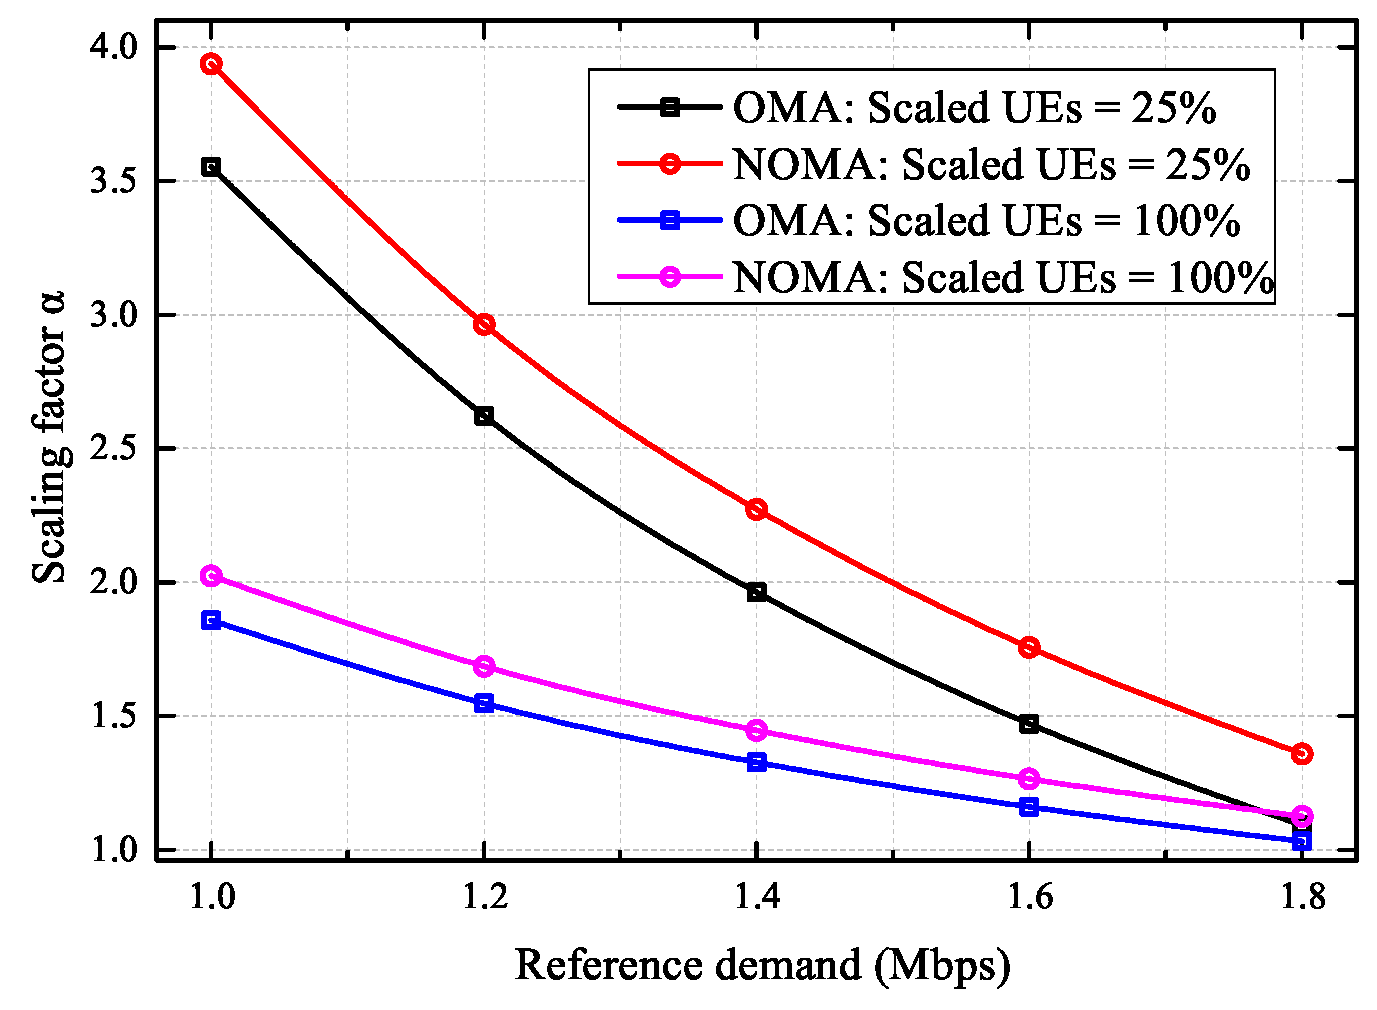
\includegraphics[width=0.5\textwidth,height=6cm]{1.eps}
\caption{This figure shows the scaling factor $\alpha$ as function of UE reference demand with different percentage of scaled UEs}
\label{1}
\end{figure}

\begin{figure}
\centering
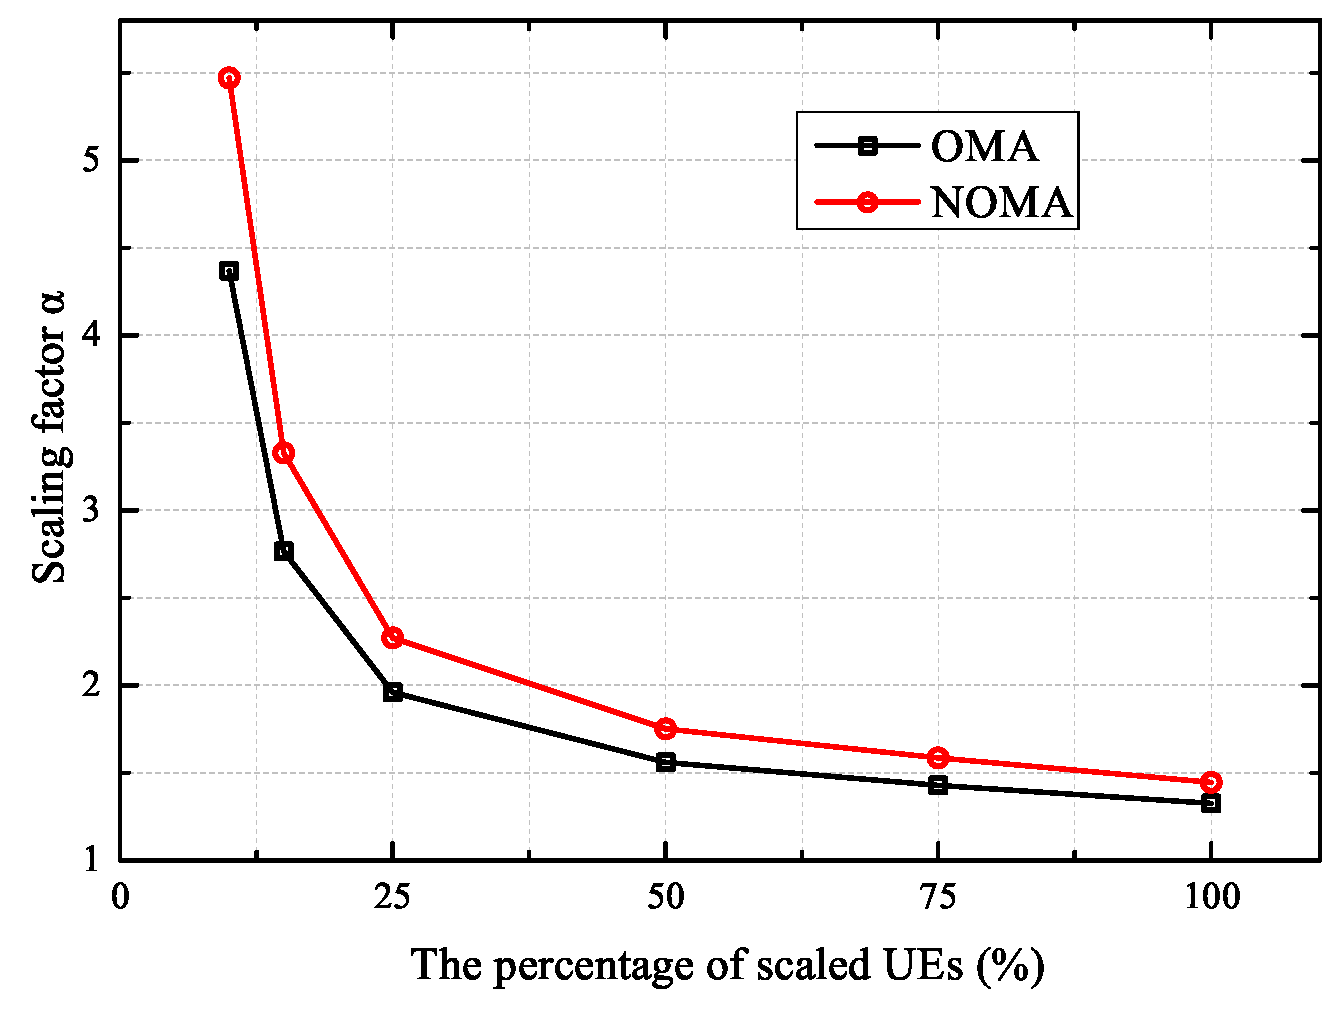
\includegraphics[width=0.5\textwidth,height=6cm]{2.eps}
\caption{This figure shows the scaling factor $\alpha$ as function of the percentage of scaled UEs with $d=1.4$ Mbps.}
\label{2}
\end{figure}

\begin{figure}
\centering
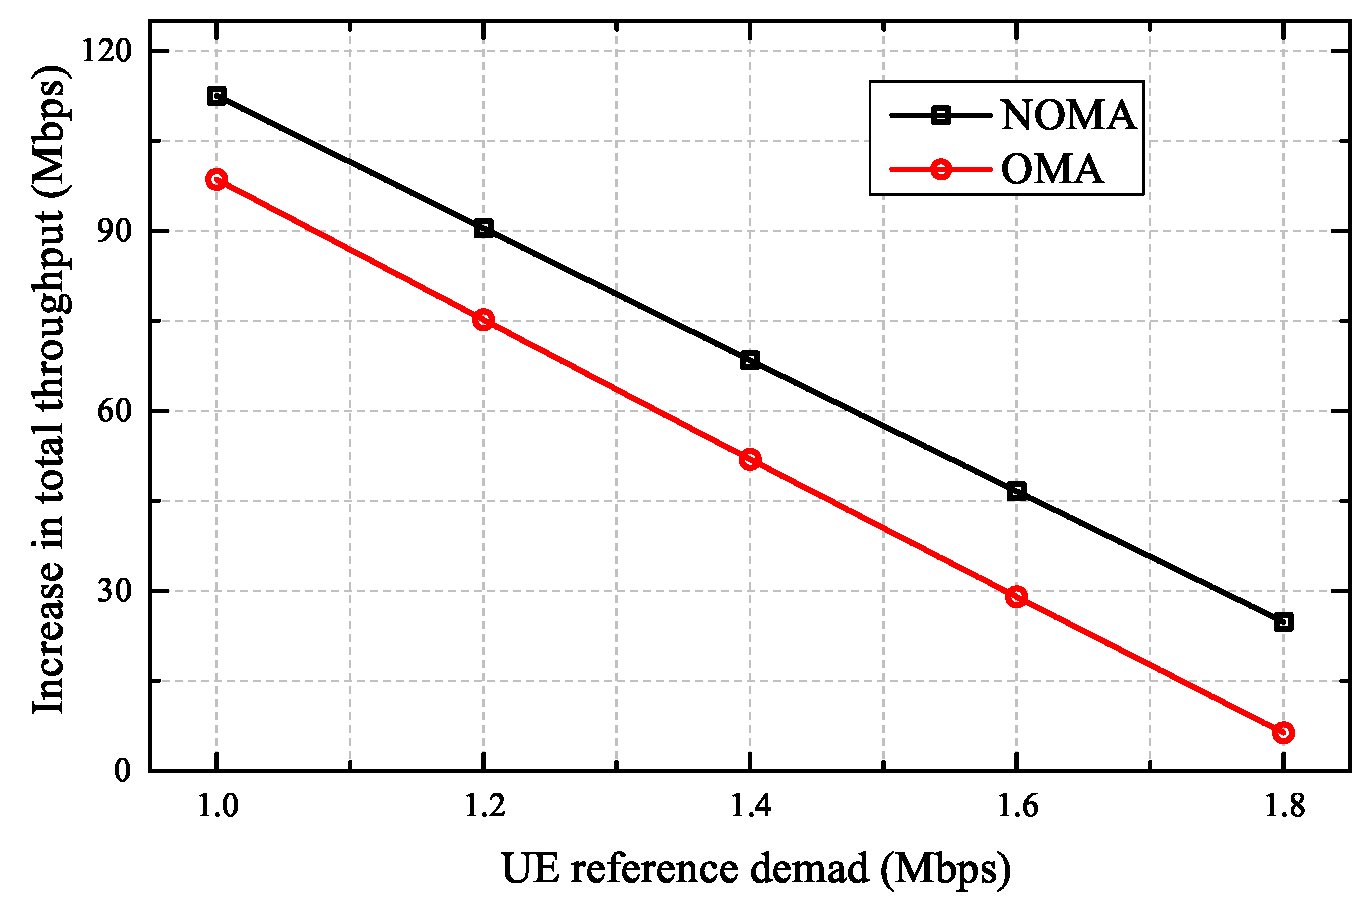
\includegraphics[width=0.5\textwidth,height=6cm]{3.eps}
\caption{This figure shows the increase in total throughput as function of UE reference demand with $P = 15$.}
\label{3}
\end{figure}

\begin{figure}
\centering
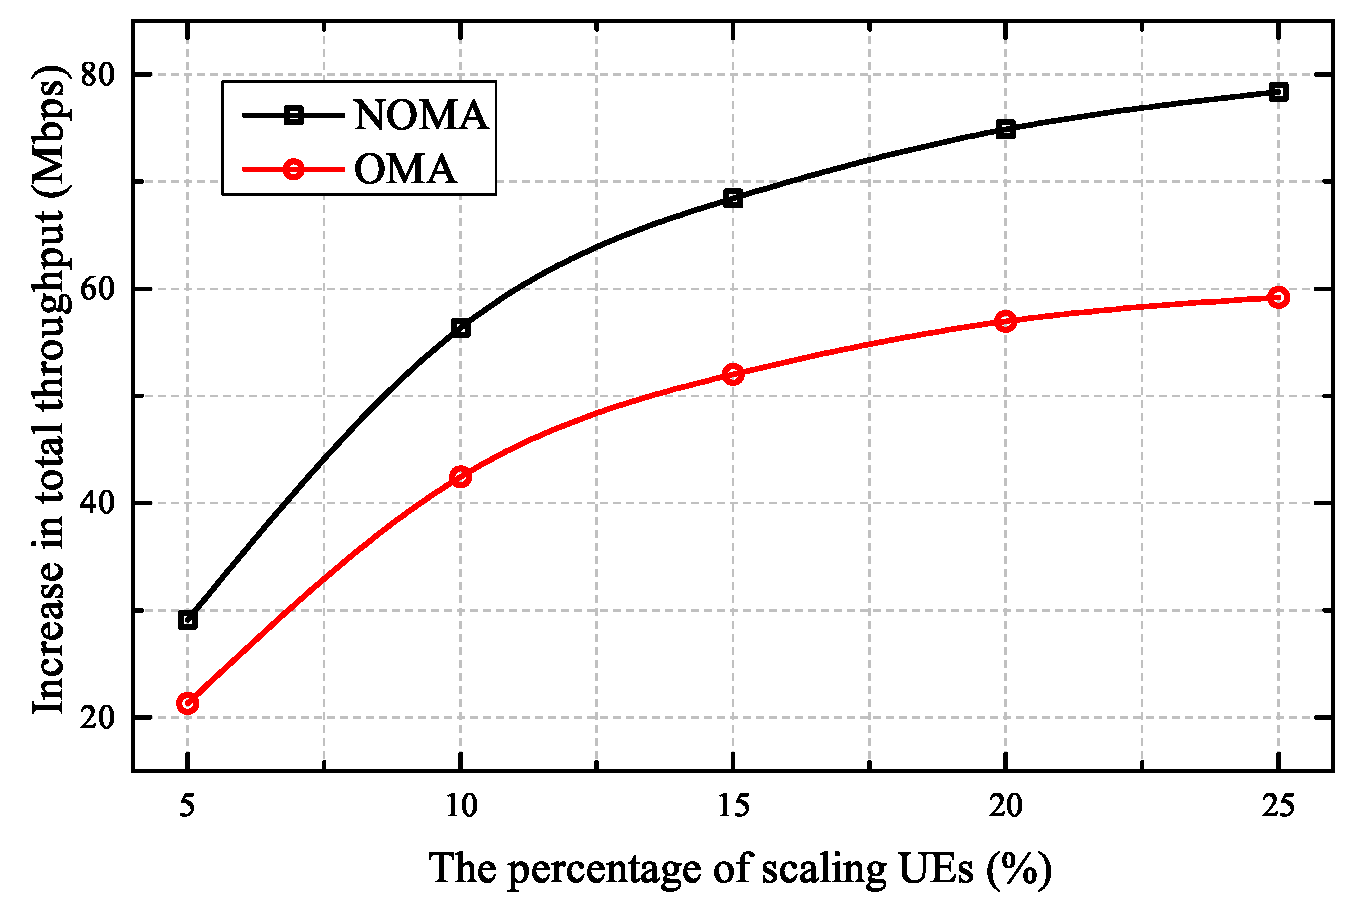
\includegraphics[width=0.5\textwidth,height=6cm]{4.eps}
\caption{This figure shows the increase in total throughput as function of UE reference demand with $d = 1.4$ Mbps.}
\label{4}
\end{figure}
%----------------------------------------------------------------------------------------------------------------------------
\begin{thebibliography}{99}

\bibitem{Do1}  T. N. Do, D. B. da Costa, T. Q. Duong and B. An, ``Improving the performance of cell-edge users in MISO-NOMA systems using TAS and SWIPT-based cooperative transmissions," {\em IEEE Transactions on Green Communications and Networking}, vol 2, no. 1, pp. 49-62, 2017.

\bibitem{Do2} T. N. Do, D. B. da Costa, T. Q. Duong and B. An, ``Improving the performance of cell-edge users in NOMA systems using cooperative relaying," {\em IEEE Transactions on Communications}, vol. 66, no. 5, pp. 1883-1901, 2018.

\bibitem{Guo} Q. Guo, C. W. Sung, Y. Chen, and C. S. Chen, ``Power control for coordinated NOMA downlink with cell-edge users", {\em IEEE Wireless Communications and Networking Conference (WCNC)}, 2018, pp. 1-6.

\bibitem{Pei} X. Pei, M. Wen and H. Yu, ``NOMA-based coordinated direct and relay system with multiple cell-edge users",  {\em IEEE International Workshop on Signal Processing Advances in Wireless Communications (SPAWC)}, 2019, pp. 1-5.

\bibitem{Ali} M. S. Ali, E. Hossain, A. Al-Dweik, and D. I. Kim, ``Downlink power allocation for CoMP-NOMA in
multi-cell networks," {\em IEEE Transactions on Communications}, vol. 66, no. 9, pp. 3982-3998, 2018. 

\bibitem{You1} L. You, D. Yuan, L. Lei, S. Sun, S. Chatzinotas, and B. Ottersten, ``Resource optimization with load coupling in multi-cell NOMA," {\em IEEE Transactions on Wireless Communications}, vol. 17, no.7, pp. 4735-4749, 2018.

\bibitem{You2} L. You and D. Yuan, ``A note on decoding order in optimizing multi-cell NOMA," {\em arXiv.org}, 2020. [Online]. Available: https://arxiv.org/abs/1909.08651.pdf

\bibitem{Ni} D. Ni, L. Hao, Q. T. Tran and X. Qian, ``Transmit power minimization for downlink multi-cell multi-carrier NOMA networks," {\em IEEE Communications Letters}, vol. 22, no. 12, pp. 2459-2462, 2018.

\bibitem{Lei} L. Lei, L. You, Y. Yang, D. Yuan, S. Chatzinotas and B. Ottersten, ``Load coupling and energy optimization in multi-cell and multi-carrier NOMA networks," {\em  IEEE Transactions on Vehicular Technology}, vol. 68, no. 11, pp.11323-11337, 2019.

\bibitem{Dai} L. Dai, B. Wang, Y. Yuan, S. Han, C. l. I, and Z. Wang, ``Non-orthogonal multiple access for 5G: solutions, challenges, opportunities, and future research trends," {\em IEEE Communications Magazine}, vol. 53, no. 9, pp. 74-81, 2015.

\bibitem{Islam} S. M. R. Islam, N. Avazov, O. A. Dobre, and K. S. Kwak, ``Power- domain non-orthogonal multiple access (NOMA) in 5G systems: Potentials and challenges," {\em IEEE Communications Surveys Tutorials}, vol. 19, no. 2, pp. 721-742, 2017.

\bibitem{41} D. Tse and P. Viswanath, {\em Fundamentals of Wireless Communication}. Cambridge university press, 2005.

\bibitem{48} ``IEC 80000-13:2008, quantities and units part 13: Information science and technology," International Electrotechnical Commission, 2008.

\bibitem{Yates} R. D. Yates, ``A framework for uplink power control in cellular radio
systems," {\em IEEE Journal on Selected Areas in Communications}, vol. 13,
no. 7, pp. 1341-1347, 1995.



\end{thebibliography}

\end{document}

